\documentclass[11pt,a4paper]{article}
\usepackage[T1]{fontenc}
\usepackage[utf8]{inputenc}
\usepackage[polish]{babel}
\usepackage{lmodern}
\usepackage[a4paper,margin=2.5cm]{geometry}
\usepackage{graphicx}
\usepackage{booktabs}
\usepackage{amsmath}
\usepackage{xcolor}
\usepackage{listings}
\usepackage{caption}
\usepackage[colorlinks=true,linkcolor=blue!50!black,citecolor=blue!50!black,urlcolor=blue!50!black]{hyperref}
\usepackage{float}

\captionsetup{font=small,labelfont=bf}
\captionsetup[table]{position=above}
\captionsetup[figure]{position=below}

\definecolor{kwcol}{RGB}{40,60,130}
\definecolor{cmcol}{RGB}{90,120,90}
\definecolor{nrcol}{RGB}{130,130,130}
\definecolor{bgcol}{RGB}{248,248,248}

\lstdefinestyle{c}{
  language=C,
  basicstyle=\ttfamily\scriptsize,
  keywordstyle=\color{kwcol},
  commentstyle=\color{cmcol}\itshape,
  stringstyle=\color{brown!70!black},
  numbers=left,
  numberstyle=\tiny\color{nrcol},
  numbersep=6pt,
  backgroundcolor=\color{bgcol},
  frame=single,
  rulecolor=\color{nrcol!50},
  breaklines=true,
  showstringspaces=false,
  tabsize=4,
  columns=fullflexible,
  keepspaces=true,
  literate={ą}{{\k{a}}}1 {ć}{{\'c}}1 {ę}{{\k{e}}}1 {ł}{{\l}}1 {ń}{{\'n}}1
           {ó}{{\'o}}1 {ś}{{\'s}}1 {ź}{{\'z}}1 {ż}{{\.z}}1
           {Ą}{{\k{A}}}1 {Ć}{{\'C}}1 {Ę}{{\k{E}}}1 {Ł}{{\L}}1 {Ń}{{\'N}}1
           {Ó}{{\'O}}1 {Ś}{{\'S}}1 {Ź}{{\'Z}}1 {Ż}{{\.Z}}1
           {„}{{,,}}1 {”}{{''}}1 {→}{{$\to$}}1,
}
\lstdefinestyle{plain}{style=c,language={},numbers=none}
\lstset{style=c}

\newcommand{\powtorzenia}{30}
\newcommand{\malyPdwa}{95}
\newcommand{\malyPosiem}{108}
\newcommand{\duzyPdwa}{79,1}
\newcommand{\duzyPosiem}{90,5}


\title{Laboratorium 4: przesyłanie komunikatów w MPI}
\author{Jakub Balicki}
\date{2026-11}

\begin{document}
\maketitle
\vspace{-1em}

\section{Środowisko i program przykładowy}
Wszystkie programy uruchamiałem na jednym komputerze: AMD Ryzen 7 5700X (8 rdzeni, 16 wątków sprzętowych), Kubuntu, Open MPI 5.0.10, \texttt{mpicc -O2 -Wall -Wextra}. Kompilacja i uruchamianie są w \texttt{Makefile}: \texttt{make} buduje programy, cele \texttt{run\_przyklad}, \texttt{run\_ring} i \texttt{run\_bcast} uruchamiają je z przykładowym wejściem, \texttt{benchmark} wykonuje pomiary, a \texttt{results} zapisuje wyniki programów do \texttt{results.txt}.

W materiałach do laboratorium nie było pliku z programem przykładowym, więc jako \texttt{przyklad.c} użyłem programu z wykładu~3 (\texttt{MPI\_Init}, \texttt{MPI\_Comm\_rank}, \texttt{MPI\_Comm\_size}, \texttt{MPI\_Finalize}), uzupełnionego o \texttt{MPI\_Get\_processor\_name}. Polecenia z treści zadania:
\begin{lstlisting}[style=plain]
mpicc przyklad.c -o prz_mpi
mpirun -np 7 --display-map ./prz_mpi
\end{lstlisting}
Fragment wyniku (pełny w \texttt{results.txt}):
\begin{lstlisting}[style=plain]
Data for node: Kubuntu-PC	Num slots: 8	Max slots: 0	Num procs: 7
    Process jobid: prterun-Kubuntu-PC-486862@1 App: 0 Process rank: 0 Bound: package[0][core:L0]
    ...
    Process jobid: prterun-Kubuntu-PC-486862@1 App: 0 Process rank: 6 Bound: package[0][core:L6]
Moj numer 5, w grupie 7 procesow, wezel Kubuntu-PC
Moj numer 6, w grupie 7 procesow, wezel Kubuntu-PC
...
Moj numer 2, w grupie 7 procesow, wezel Kubuntu-PC
\end{lstlisting}
Mapa procesów (\texttt{-{}-display-map}) pokazuje jeden węzeł z 8 slotami (po jednym na rdzeń fizyczny), a każdy proces jest przypięty do osobnego rdzenia. Dlatego bez \texttt{-{}-oversubscribe} można uruchomić najwyżej 8 procesów. Kolejność wierszy \texttt{Moj numer \ldots} zmienia się między uruchomieniami, bo procesy piszą niezależnie, a \texttt{mpirun} przekazuje ich wyjście w kolejności nadejścia.

\section{Pierścień}
Proces~0 wczytuje liczbę i wysyła ją do procesu~1, proces $i$ odbiera od $i-1$ i wysyła do $(i+1) \bmod p$, więc ostatni odsyła liczbę do procesu~0. Liczba ujemna też obiega cały pierścień, ale nikt jej nie wypisuje; dzięki temu każdy proces kończy pętlę i nikt nie zostaje zablokowany w \texttt{MPI\_Recv}.
\lstinputlisting[firstline=31,lastline=54,firstnumber=31]{../ring.c}
\begin{lstlisting}[style=plain]
$ printf "5\n7\n-1\n" | mpirun -np 8 ./ring
Podaj liczbę:
Proces 1 dostal 5 od procesu 0
Proces 2 dostal 5 od procesu 1
...
Proces 7 dostal 5 od procesu 6
Proces 0 dostal 5 od procesu 7
Podaj liczbę:
Proces 1 dostal 7 od procesu 0
...
Proces 0 dostal 7 od procesu 7
Podaj liczbę:
\end{lstlisting}
W kolejnych uruchomieniach wydruki pojawiały się w tej samej kolejności, bo proces wypisuje dopiero po odebraniu liczby, a poprzedni proces wypisał przed jej wysłaniem.

\section{Rozgłaszanie przez \texttt{MPI\_Bcast}}
\lstinputlisting[firstline=20,lastline=36,firstnumber=20]{../bcast.c}
\begin{lstlisting}[style=plain]
$ printf "5\n7\n-1\n" | mpirun -np 4 ./bcast
Podaj liczbę:
Proces 0 z 4 otrzymal liczbe 5
Podaj liczbę:
Proces 0 z 4 otrzymal liczbe 7
Podaj liczbę:
Proces 1 z 4 otrzymal liczbe 5
Proces 1 z 4 otrzymal liczbe 7
Proces 3 z 4 otrzymal liczbe 5
...
\end{lstlisting}
Każdy proces dostaje obie liczby, ale wydruki różnych procesów się przeplatają: \texttt{MPI\_Bcast} nie synchronizuje procesów po zakończeniu i proces~0 może od razu poprosić o kolejną liczbę.

\section{Suma tablicy przez Scatter i Gather}
Proces~0 tworzy tablicę $N=10\,000$ liczb całkowitych z przedziału 0--100 (\texttt{srand(42)}, \texttt{rand() \% 101}). Treść zadania zakłada równe części, ale $10\,000$ nie dzieli się przez 3, 6 i 7. Dlatego dla takich $p$ używam \texttt{MPI\_Scatterv}: tablica \texttt{counts} mówi, ile elementów dostaje każdy proces (pierwsze $N \bmod p$ procesów o jeden więcej), a \texttt{displs} -- od którego indeksu zaczyna się jego część. Dla $p$ = 2, 4, 5, 8 podział jest równy i program wywołuje zwykłe \texttt{MPI\_Scatter}. Każdy proces liczy sumę swojej części, \texttt{MPI\_Gather} zbiera sumy w procesie~0, który dodaje je i porównuje z sumą policzoną sekwencyjnie z całej tablicy.
\lstinputlisting[firstline=50,lastline=82,firstnumber=50]{../scatter_gather.c}

Czas mierzę od chwili zaraz po \texttt{MPI\_Init} do końca \texttt{MPI\_Gather} (samo \texttt{MPI\_Init} nie jest wliczone, bo przed nim nie można wywołać \texttt{MPI\_Wtime}). W tym przedziale jest też generowanie tablicy w procesie~0. \texttt{MPI\_Barrier} na początku wyrównuje start procesów, a jako wynik biorę najdłuższy z czasów procesów (\texttt{MPI\_Reduce} z \texttt{MPI\_MAX}), czyli czas, po którym wszystkie procesy skończyły komunikację.
\begin{lstlisting}[style=plain]
$ mpirun -np 7 ./scatter_gather
Liczba procesów: 7, N = 10000, MPI_Scatterv
Proces 0: 1429 elementów, suma 72944
Proces 1: 1429 elementów, suma 71693
...
Proces 6: 1428 elementów, suma 69737
Suma całkowita: 494615 (sekwencyjnie 494615) OK
Czas: 0.000208 s
\end{lstlisting}

\subsection*{Pomiary}
Skrypt \texttt{run\_benchmark.sh} uruchamia program dla $p=2,\dots,8$: najpierw jedno uruchomienie rozgrzewkowe (pomijane), potem \powtorzenia{} osobnych uruchomień \texttt{mpirun}. Surowe wyniki są w \texttt{results\_raw.csv}; we wszystkich wierszach suma zgadza się z sekwencyjną. Dla porównania ten sam pomiar wykonałem dla $N=10^7$ (\texttt{results\_raw\_duze.csv}). W czasie pomiarów na komputerze działały też inne procesy użytkownika (m.in.\ trening sieci neuronowej), co tłumaczy pojedyncze wartości maksymalne odstające od mediany.

\begin{table}[H]
\centering
\caption{Czas od \texttt{MPI\_Init} do końca \texttt{MPI\_Gather}: mediana, minimum i maksimum z \powtorzenia{} uruchomień. Pomiar lokalny (jeden komputer).}\label{tab:czasy}
\begin{tabular}{rrrrrrr}
\toprule
 & \multicolumn{3}{c}{$N=10\,000$ [$\mu$s]} & \multicolumn{3}{c}{$N=10^7$ [ms]} \\
\cmidrule(lr){2-4}\cmidrule(lr){5-7}
$p$ & mediana & min & max & mediana & min & max \\
\midrule
2 & 94 & 92 & 179 & 79,16 & 77,13 & 83,40 \\
3 & 93 & 91 & 145 & 79,06 & 78,55 & 84,93 \\
4 & 106 & 98 & 278 & 80,83 & 79,56 & 151,52 \\
5 & 102 & 98 & 129 & 85,27 & 80,00 & 99,33 \\
6 & 122 & 115 & 150 & 83,59 & 82,48 & 103,00 \\
7 & 145 & 116 & 172 & 87,30 & 86,28 & 90,75 \\
8 & 132 & 110 & 245 & 90,08 & 89,14 & 132,26 \\
\bottomrule
\end{tabular}

\end{table}

\begin{figure}[H]
\centering
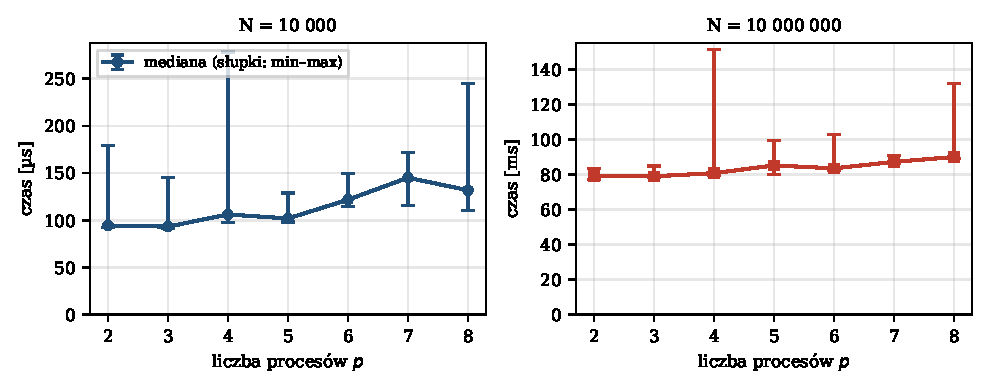
\includegraphics[width=0.95\textwidth]{fig_czas.pdf}
\caption{Czas wykonania względem liczby procesów (mediana, słupki od minimum do maksimum).}\label{fig:czas}
\end{figure}

\section{Wnioski}
\begin{itemize}
\item Dla $N=10\,000$ czas rośnie z liczbą procesów: mediana wynosi \malyPdwa{}\,$\mu$s dla $p=2$ i \malyPosiem{}\,$\mu$s dla $p=8$. Samo sumowanie 10\,000 liczb jest bardzo krótkie, więc o czasie decyduje komunikacja (bariera, Scatter, Gather), a jej koszt rośnie z liczbą uczestników operacji zbiorowych.
\item Dla $N=10^7$ czas też nie spada (\duzyPdwa{}\,ms dla $p=2$, \duzyPosiem{}\,ms dla $p=8$). Prawie stały czas wskazuje, że przeważają kroki wykonywane tylko przez proces~0: generowanie tablicy i wysłanie jej części do pozostałych procesów. Równolegle liczona jest tylko suma lokalna, więc zwiększanie $p$ skraca niewielką część całego czasu.
\item Rozdzielanie danych przez MPI opłaca się dopiero wtedy, gdy obliczenia na jeden element są dużo droższe niż jego przesłanie albo gdy dane powstają od razu w procesach (bez rozsyłania z procesu~0).
\item Pomiar jest lokalny: procesy komunikują się przez pamięć współdzieloną jednego komputera. Na kilku węzłach połączonych siecią narzut komunikacji byłby większy.
\item Rozrzut wyników jest mały w porównaniu z medianą poza pojedynczymi uruchomieniami (maksima w tabeli), które przypisuję innym procesom działającym w tym czasie; dlatego porównuję mediany.
\end{itemize}

\appendix
\section{Pełny kod źródłowy}
\subsection*{\texttt{przyklad.c}}
\lstinputlisting{../przyklad.c}
\subsection*{\texttt{ring.c}}
\lstinputlisting{../ring.c}
\subsection*{\texttt{bcast.c}}
\lstinputlisting{../bcast.c}
\subsection*{\texttt{scatter\_gather.c}}
\lstinputlisting{../scatter_gather.c}

\end{document}
